\documentclass[]{book}
\usepackage{lmodern}
\usepackage{amssymb,amsmath}
\usepackage{ifxetex,ifluatex}
\usepackage{fixltx2e} % provides \textsubscript
\ifnum 0\ifxetex 1\fi\ifluatex 1\fi=0 % if pdftex
  \usepackage[T1]{fontenc}
  \usepackage[utf8]{inputenc}
\else % if luatex or xelatex
  \ifxetex
    \usepackage{mathspec}
  \else
    \usepackage{fontspec}
  \fi
  \defaultfontfeatures{Ligatures=TeX,Scale=MatchLowercase}
\fi
% use upquote if available, for straight quotes in verbatim environments
\IfFileExists{upquote.sty}{\usepackage{upquote}}{}
% use microtype if available
\IfFileExists{microtype.sty}{%
\usepackage{microtype}
\UseMicrotypeSet[protrusion]{basicmath} % disable protrusion for tt fonts
}{}
\usepackage[margin=1in]{geometry}
\usepackage{hyperref}
\hypersetup{unicode=true,
            pdftitle={Immunogenicity - Tiered Approuch to Assess ADA Positive Samples},
            pdfauthor={Phil Bowsher},
            pdfborder={0 0 0},
            breaklinks=true}
\urlstyle{same}  % don't use monospace font for urls
\usepackage{natbib}
\bibliographystyle{apalike}
\usepackage{color}
\usepackage{fancyvrb}
\newcommand{\VerbBar}{|}
\newcommand{\VERB}{\Verb[commandchars=\\\{\}]}
\DefineVerbatimEnvironment{Highlighting}{Verbatim}{commandchars=\\\{\}}
% Add ',fontsize=\small' for more characters per line
\usepackage{framed}
\definecolor{shadecolor}{RGB}{248,248,248}
\newenvironment{Shaded}{\begin{snugshade}}{\end{snugshade}}
\newcommand{\KeywordTok}[1]{\textcolor[rgb]{0.13,0.29,0.53}{\textbf{{#1}}}}
\newcommand{\DataTypeTok}[1]{\textcolor[rgb]{0.13,0.29,0.53}{{#1}}}
\newcommand{\DecValTok}[1]{\textcolor[rgb]{0.00,0.00,0.81}{{#1}}}
\newcommand{\BaseNTok}[1]{\textcolor[rgb]{0.00,0.00,0.81}{{#1}}}
\newcommand{\FloatTok}[1]{\textcolor[rgb]{0.00,0.00,0.81}{{#1}}}
\newcommand{\ConstantTok}[1]{\textcolor[rgb]{0.00,0.00,0.00}{{#1}}}
\newcommand{\CharTok}[1]{\textcolor[rgb]{0.31,0.60,0.02}{{#1}}}
\newcommand{\SpecialCharTok}[1]{\textcolor[rgb]{0.00,0.00,0.00}{{#1}}}
\newcommand{\StringTok}[1]{\textcolor[rgb]{0.31,0.60,0.02}{{#1}}}
\newcommand{\VerbatimStringTok}[1]{\textcolor[rgb]{0.31,0.60,0.02}{{#1}}}
\newcommand{\SpecialStringTok}[1]{\textcolor[rgb]{0.31,0.60,0.02}{{#1}}}
\newcommand{\ImportTok}[1]{{#1}}
\newcommand{\CommentTok}[1]{\textcolor[rgb]{0.56,0.35,0.01}{\textit{{#1}}}}
\newcommand{\DocumentationTok}[1]{\textcolor[rgb]{0.56,0.35,0.01}{\textbf{\textit{{#1}}}}}
\newcommand{\AnnotationTok}[1]{\textcolor[rgb]{0.56,0.35,0.01}{\textbf{\textit{{#1}}}}}
\newcommand{\CommentVarTok}[1]{\textcolor[rgb]{0.56,0.35,0.01}{\textbf{\textit{{#1}}}}}
\newcommand{\OtherTok}[1]{\textcolor[rgb]{0.56,0.35,0.01}{{#1}}}
\newcommand{\FunctionTok}[1]{\textcolor[rgb]{0.00,0.00,0.00}{{#1}}}
\newcommand{\VariableTok}[1]{\textcolor[rgb]{0.00,0.00,0.00}{{#1}}}
\newcommand{\ControlFlowTok}[1]{\textcolor[rgb]{0.13,0.29,0.53}{\textbf{{#1}}}}
\newcommand{\OperatorTok}[1]{\textcolor[rgb]{0.81,0.36,0.00}{\textbf{{#1}}}}
\newcommand{\BuiltInTok}[1]{{#1}}
\newcommand{\ExtensionTok}[1]{{#1}}
\newcommand{\PreprocessorTok}[1]{\textcolor[rgb]{0.56,0.35,0.01}{\textit{{#1}}}}
\newcommand{\AttributeTok}[1]{\textcolor[rgb]{0.77,0.63,0.00}{{#1}}}
\newcommand{\RegionMarkerTok}[1]{{#1}}
\newcommand{\InformationTok}[1]{\textcolor[rgb]{0.56,0.35,0.01}{\textbf{\textit{{#1}}}}}
\newcommand{\WarningTok}[1]{\textcolor[rgb]{0.56,0.35,0.01}{\textbf{\textit{{#1}}}}}
\newcommand{\AlertTok}[1]{\textcolor[rgb]{0.94,0.16,0.16}{{#1}}}
\newcommand{\ErrorTok}[1]{\textcolor[rgb]{0.64,0.00,0.00}{\textbf{{#1}}}}
\newcommand{\NormalTok}[1]{{#1}}
\usepackage{longtable,booktabs}
\usepackage{graphicx,grffile}
\makeatletter
\def\maxwidth{\ifdim\Gin@nat@width>\linewidth\linewidth\else\Gin@nat@width\fi}
\def\maxheight{\ifdim\Gin@nat@height>\textheight\textheight\else\Gin@nat@height\fi}
\makeatother
% Scale images if necessary, so that they will not overflow the page
% margins by default, and it is still possible to overwrite the defaults
% using explicit options in \includegraphics[width, height, ...]{}
\setkeys{Gin}{width=\maxwidth,height=\maxheight,keepaspectratio}
\IfFileExists{parskip.sty}{%
\usepackage{parskip}
}{% else
\setlength{\parindent}{0pt}
\setlength{\parskip}{6pt plus 2pt minus 1pt}
}
\setlength{\emergencystretch}{3em}  % prevent overfull lines
\providecommand{\tightlist}{%
  \setlength{\itemsep}{0pt}\setlength{\parskip}{0pt}}
\setcounter{secnumdepth}{5}
% Redefines (sub)paragraphs to behave more like sections
\ifx\paragraph\undefined\else
\let\oldparagraph\paragraph
\renewcommand{\paragraph}[1]{\oldparagraph{#1}\mbox{}}
\fi
\ifx\subparagraph\undefined\else
\let\oldsubparagraph\subparagraph
\renewcommand{\subparagraph}[1]{\oldsubparagraph{#1}\mbox{}}
\fi

%%% Use protect on footnotes to avoid problems with footnotes in titles
\let\rmarkdownfootnote\footnote%
\def\footnote{\protect\rmarkdownfootnote}

%%% Change title format to be more compact
\usepackage{titling}

% Create subtitle command for use in maketitle
\newcommand{\subtitle}[1]{
  \posttitle{
    \begin{center}\large#1\end{center}
    }
}

\setlength{\droptitle}{-2em}
  \title{Immunogenicity - Tiered Approuch to Assess ADA Positive Samples}
  \pretitle{\vspace{\droptitle}\centering\huge}
  \posttitle{\par}
  \author{Phil Bowsher}
  \preauthor{\centering\large\emph}
  \postauthor{\par}
  \predate{\centering\large\emph}
  \postdate{\par}
  \date{2017-05-12}

\usepackage{booktabs}
\usepackage{amsthm}
\makeatletter
\def\thm@space@setup{%
  \thm@preskip=8pt plus 2pt minus 4pt
  \thm@postskip=\thm@preskip
}
\makeatother

\begin{document}
\maketitle

{
\setcounter{tocdepth}{1}
\tableofcontents
}
\chapter{Prerequisites}\label{prerequisites}

This is a \emph{sample} book written in \textbf{Markdown}. You can use
anything that Pandoc's Markdown supports, e.g., a math equation
\(a^2 + b^2 = c^2\).

For now, you have to install the development versions of
\textbf{bookdown} from Github:

\begin{Shaded}
\begin{Highlighting}[]
\NormalTok{devtools::}\KeywordTok{install_github}\NormalTok{(}\StringTok{"rstudio/bookdown"}\NormalTok{)}
\end{Highlighting}
\end{Shaded}

Remember each Rmd file contains one and only one chapter, and a chapter
is defined by the first-level heading \texttt{\#}.

To compile this example to PDF, you need to install XeLaTeX.

\chapter{Introduction}\label{intro}

\section{Study Information}\label{study-information}

\begin{itemize}
\tightlist
\item
  Client name: Adello biologics, LLC (Formerly known as Therapeutic
  Proteins, LLC)
\item
  Celerion Study No. CA18641
\end{itemize}

\textbf{NOTE FROM BIN (1)}: in the experiment, subjects will undergo the
following steps (in order):

\begin{itemize}
\tightlist
\item
  \textbf{\emph{ADA screening test}}. If the screening result is
  \emph{NEGATIVE}, then the result will be recoreded \emph{NEGATIVE},
  otherwise screening \emph{POSITIVE} and continue
\item
  \textbf{\emph{ADA confirmatory test}}. If the result is
  \emph{NEGATIVE}, then the subject will have a confirmatory
  \emph{NEGATIVE} result, otherwise a \emph{POSITIVE} result with a
  ``titer'' value recorded and continue
\item
  \textbf{\emph{ADA neutralizing test}}. If the result is
  \emph{NEGATIVE}, then the subject will have a neutralizing
  \emph{NEGATIVE} result, otherwise \emph{POSITIVE} with a ``titer''
  value recorded and there will be no more test.
\end{itemize}

\textbf{NOTE FROM BIN (2)}: The cut-off value to determine whether a
subject has \emph{POSITIVE} or \emph{NEGATIVE} ADA result may be
different (per assay). Therefore, when (if needed) analyzing titer
results, there should be a batch effect.

\begin{Shaded}
\begin{Highlighting}[]
\KeywordTok{par}\NormalTok{(}\DataTypeTok{mar =} \KeywordTok{c}\NormalTok{(}\DecValTok{4}\NormalTok{, }\DecValTok{4}\NormalTok{, .}\DecValTok{1}\NormalTok{, .}\DecValTok{1}\NormalTok{))}
\KeywordTok{plot}\NormalTok{(pressure, }\DataTypeTok{type =} \StringTok{'b'}\NormalTok{, }\DataTypeTok{pch =} \DecValTok{19}\NormalTok{)}
\end{Highlighting}
\end{Shaded}

\begin{figure}

{\centering 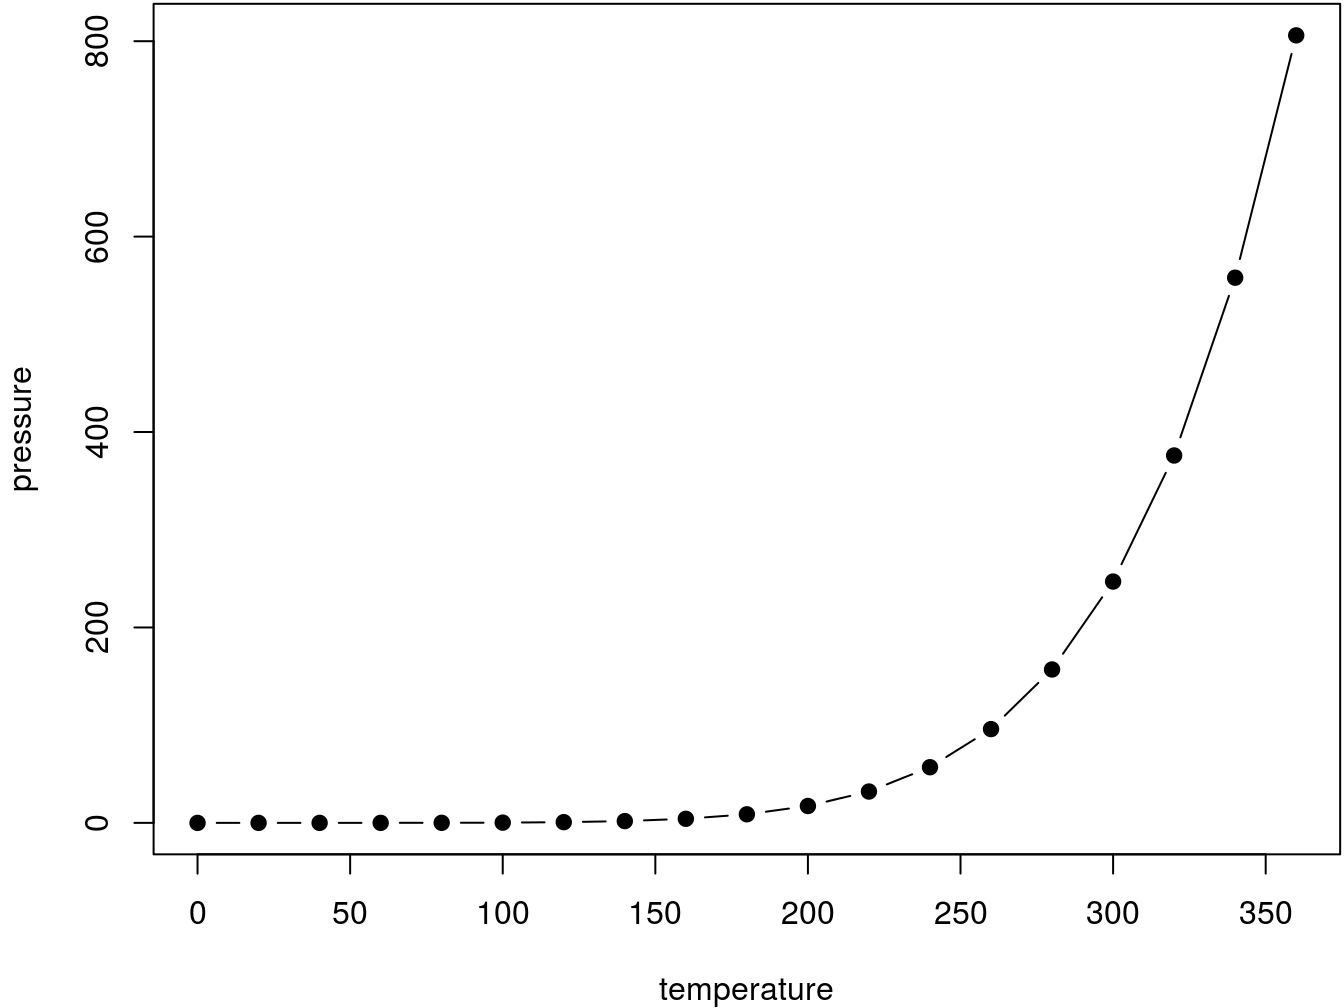
\includegraphics[width=0.8\linewidth]{bookdown-demo_files/figure-latex/nice-fig-1} 

}

\caption{Here is a nice figure!}\label{fig:nice-fig}
\end{figure}

Reference a figure by its code chunk label with the \texttt{fig:}
prefix, e.g., see Figure \ref{fig:nice-fig}. Similarly, you can
reference tables generated from \texttt{knitr::kable()}, e.g., see Table
\ref{tab:nice-tab}.

\begin{Shaded}
\begin{Highlighting}[]
\NormalTok{knitr::}\KeywordTok{kable}\NormalTok{(}
  \KeywordTok{head}\NormalTok{(iris, }\DecValTok{20}\NormalTok{), }\DataTypeTok{caption =} \StringTok{'Here is a nice table!'}\NormalTok{,}
  \DataTypeTok{booktabs =} \OtherTok{TRUE}
\NormalTok{)}
\end{Highlighting}
\end{Shaded}

\begin{table}

\caption{\label{tab:nice-tab}Here is a nice table!}
\centering
\begin{tabular}[t]{rrrrl}
\toprule
Sepal.Length & Sepal.Width & Petal.Length & Petal.Width & Species\\
\midrule
5.1 & 3.5 & 1.4 & 0.2 & setosa\\
4.9 & 3.0 & 1.4 & 0.2 & setosa\\
4.7 & 3.2 & 1.3 & 0.2 & setosa\\
4.6 & 3.1 & 1.5 & 0.2 & setosa\\
5.0 & 3.6 & 1.4 & 0.2 & setosa\\
\addlinespace
5.4 & 3.9 & 1.7 & 0.4 & setosa\\
4.6 & 3.4 & 1.4 & 0.3 & setosa\\
5.0 & 3.4 & 1.5 & 0.2 & setosa\\
4.4 & 2.9 & 1.4 & 0.2 & setosa\\
4.9 & 3.1 & 1.5 & 0.1 & setosa\\
\addlinespace
5.4 & 3.7 & 1.5 & 0.2 & setosa\\
4.8 & 3.4 & 1.6 & 0.2 & setosa\\
4.8 & 3.0 & 1.4 & 0.1 & setosa\\
4.3 & 3.0 & 1.1 & 0.1 & setosa\\
5.8 & 4.0 & 1.2 & 0.2 & setosa\\
\addlinespace
5.7 & 4.4 & 1.5 & 0.4 & setosa\\
5.4 & 3.9 & 1.3 & 0.4 & setosa\\
5.1 & 3.5 & 1.4 & 0.3 & setosa\\
5.7 & 3.8 & 1.7 & 0.3 & setosa\\
5.1 & 3.8 & 1.5 & 0.3 & setosa\\
\bottomrule
\end{tabular}
\end{table}

You can write citations, too. For example, we are using the
\textbf{bookdown} package \citep{R-bookdown} in this sample book, which
was built on top of R Markdown and \textbf{knitr} \citep{xie2015}.

\chapter{Literature}\label{literature}

\section{Case Study}\label{case-study}

\url{http://bcn2016.europeanbioanalysisforum.eu/wp-content/uploads/2016/12/D2J4-4-Viswanath-Devanarayan_Abbvie.pdf}

\url{https://zerista.s3.amazonaws.com/item_files/f4b3/attachments/39608/original/aaps_nbc_2015_hendricks.pdf}

The goal of this study is to compare immunogenicity of
Theragrastim\textsuperscript{®} (new drug) and
Neupogen\textsuperscript{®} (reference drug) after multiple subcutaneous
(SC) administrations in healthy subjects. ADA levels for Theragrastim®
and Neupogen® will be estimated and compared to evaluate potential
difference between the two products in the incidence of human immune
responses.

This is a one center, single-blind, randomized, parallel, multiple-dose,
safety and immunogenicity study. A total number of one hundred thirty
four (134) healthy adult male and female subjects will be enrolled and
randomized to 1 of 2 treatments (67 subjects per treatment).

The sample size is chosen based on a target of 61 subjects per arm as
calculated, to which 6 subjects (\textasciitilde{}10\%) were added to
each arm to account for potential dropouts. With 61 subjects per arm,
the trial can show, with 80\% power, that the upper bound of the
one-sided 95\% confidence interval of the difference in ADA+ rates
between the two products is below (or above) the non-inferiority margin
(10\%)

The power calculation for sample size is based on the following
assumptions:

\begin{itemize}
\tightlist
\item
  The ADA+ rate of Neupogen\textsuperscript{®} is 3.3\%
\item
  The ADA+ rate of Theragrastim\textsuperscript{®} is 3.3\%
\item
  The mean ADA+ rate difference (\(\delta\)) between the two products is
  zero;
\item
  The NI margin (\(\delta_0\)) is 10\%.
\end{itemize}

The power calculation is based on exact method \citep{chan1999test}
using \(\delta\)-projected \(Z\)-statistic (i.e., the score statistic)
with REML estimation procedure \citep{miettinen1985comparative}.

\section{Statistical Analysis}\label{statistical-analysis}

The rate (or proportion) of subjects that have ADA+ in confimatory test
and neutralizing test (if needed) will be compared between
Theragrastim\textsuperscript{®} and Neupogen\textsuperscript{®}
treatments to determine if any differences are statistically meaningful.

\chapter{Methods}\label{methods}

\section{Background}\label{background}

Therapeutic proteins (sometimes also called biologics,
biopharmaceuticals, biological products, or biological medicinal
products) and peptides have the potential to induce immunogenicity. The
consequences of product immunogenicity vary from no evidience of
clinical effect to severe, life-threatening responses. Anti-drug
antibodies (ADA) have been implicated in infusion reactions and
anaphylaxis as well as immune complex-mediated disease. ADA have also
caused secondary treatment failures (loss of efficacy) and, in rare
occasions, more serious thrombocytopenia and pure red cell aplasia.
Therefore, ADA are a medical concern in terms of safety and long-term
efficacy of the drug and it is critical to evaluate their development in
all patients during clinical studies, not just in a symptom-driven
manner. With a goal of guiding medical practice, the elucidation of ADA
responses and their characteristics relative to clinical consequences is
vital \citep{shankar2014assessment}.

ADA comprises neutralizing and non-neutralizing ADA. Other terms that
have been used for ADA include anti-therapeutic antibody (ATA),
anti-product antibody (APA), or anti-biologic antibody (ABA).

\begin{itemize}
\tightlist
\item
  Neutralizing ADA (NAb): ADA that inhibits or reduces the
  pharmacological activity of the biologic drug molecule, as determined
  by an \emph{in vitro} test or animal-based bioassay method, regardless
  of its \emph{in vitro} clinical relavence (i.e., whether or not test
  method results relate to clinical impact in the subject).
\item
  Non-neutralizing ADA (non-neutralizing antibody, non- NAb): ADA that
  binds to the biologic drug molecule but does not inhibit its
  pharmacological activity in an in vitro test or animal-based bioassay
  method, regardless of its in vivo clinical relevance (i.e., whether or
  not test method results relate to clinical impact in the subject).
\end{itemize}

\chapter{Applications}\label{applications}

Some \emph{significant} applications are demonstrated in this chapter.

\subsection{Statistical method}\label{statistical-method}

The rate difference between Theragrastim\textsuperscript{®} and
Neupogen\textsuperscript{®} will be defined as:

\begin{equation}\label{eq:adadiff}
\delta = \pi_1 -\pi_2
\end{equation}

where \(\pi_1\) is the ADA+ rate of Theragrastim\textsuperscript{®} and
\(\pi_2\) is that of Neupogen\textsuperscript{®}.

In hypotheses testing, the research or alternative hypothesis represents
what the study aims to show. The null hypothesis is the opposite of the
research hypothesis and is what the investigator hopes to disprove
\citep{walker2011understanding}. Therefore, the primary statistical
hypothesis for the clinical trial will be tested using

\begin{equation}\label{eq:immunetest}
H_0: \pi_1 - \pi_2 \geq 0.10~~~  VS~~~~~ H_1: \pi_1 - \pi_2 < 0.1
\end{equation}

Confidence intervals (CIs) will be calculated using the
Farrington-Manning method (\(\delta\)-projected \(Z\)-statistic)
recommended by \citet{chan1999test}.

Note that in SAS, the null in Expression (\ref{eq:immunetest}) is
equivalently stated as

\begin{equation}\label{eq:immunetest2}
H_0: \pi_2 - \pi_1 \leq -0.10~~~  VS~~~~~ H_1: \pi_2 - \pi_1 > -0.1
\end{equation}

Therefore, in the SAS output, the null is rejected (i.e.,
Theragrastim\textsuperscript{®} is non-inferior to
Neupogen\textsuperscript{®} in terms of ADA+ rate) if the lower bound of
the one-sided 95\% CI of the difference is above NI margin (-0.10).

\section{Example one}\label{example-one}

\section{Example two}\label{example-two}

\chapter{Final Words}\label{final-words}

\subsection{R implementation}\label{r-implementation}

Programmer note: the above code produces results as desired only if the
input data set has the same structure as the data set created by the
following code. If not, please sort the test data by time treat and
response as this one.

\textbackslash{}end\{verbatim\}

\bibliography{packages.bib,book.bib}


\end{document}
